The LifeCycle agend was also used for cross-integration tests of all three
components (PhEDEx, DBS3, and DAS) within a controlled environment and thus
without interfering with production services. Fake data was created and injected into PhEDEx and DBS. DAS then
retrieved information about the data from both sources, and compared the
results. For an illustration of the workflow see Fig.~\ref{fig:Integ-Phedex-DBS-DAS}. By injecting specific errors in either PhEDEx or DBS (changing filenames etc)
we can fake errors that we expect to detect with DAS. Special event-handlers
are used to compare the errors detected by DAS with the injected errors, and
alert us to any unexpected failures.

In the current implementation six kinds of failure can be faked and the probability to occur
can be adjusted for each single failure type individually.

\begin{itemize}
\item Single file is skipped in the PhEDEx data
\item Single file is skipped in the DBS data
\item The checksum for a single file is changed for the PhEDEx data
\item The checksum for a single file is changed for the DBS data
\item The size for a single file is changed for the PhEDEx data
\item The size for a single file is changed for the DBS data
\end{itemize}

The payload-provider (data provider) generates fake data, which then can be
injected to a node of the LifeCycle testbed. It also
generates extensions to filenames specifying the failure type the file is
affected by (according to the probability that was specified).

Special modules read the filenames and act on all files with a certain
extension specifying the kind of failure the file is affected by. This
includes whether the PhEDEx information, the DBS information,
or both are affected and the kind of failure (different checksum, different
size or skipped file). Also combinations of these failures are possible for
one single file. According to the kind of failure these modules either
remove the files, change their size or their checksum, or perform a
combination of the mentioned actions, when injecting the
information to PhEDEx and DBS3.

After passing these error-handler modules, all files are injected into PhEDEx
and DBS and a DAS-query is performed retrieving the information on the
injected data from PhEDEx and from DBS3.
These two sets of information on the injected data are compared and the found
differences are checked against the true information on the injected failures.
In this way we can check that DAS properly reports all occuring mismatches in
the information on a certain datset coming both from PhEDEx and/or DBS3.


\begin{figure}[h]
 \centering
   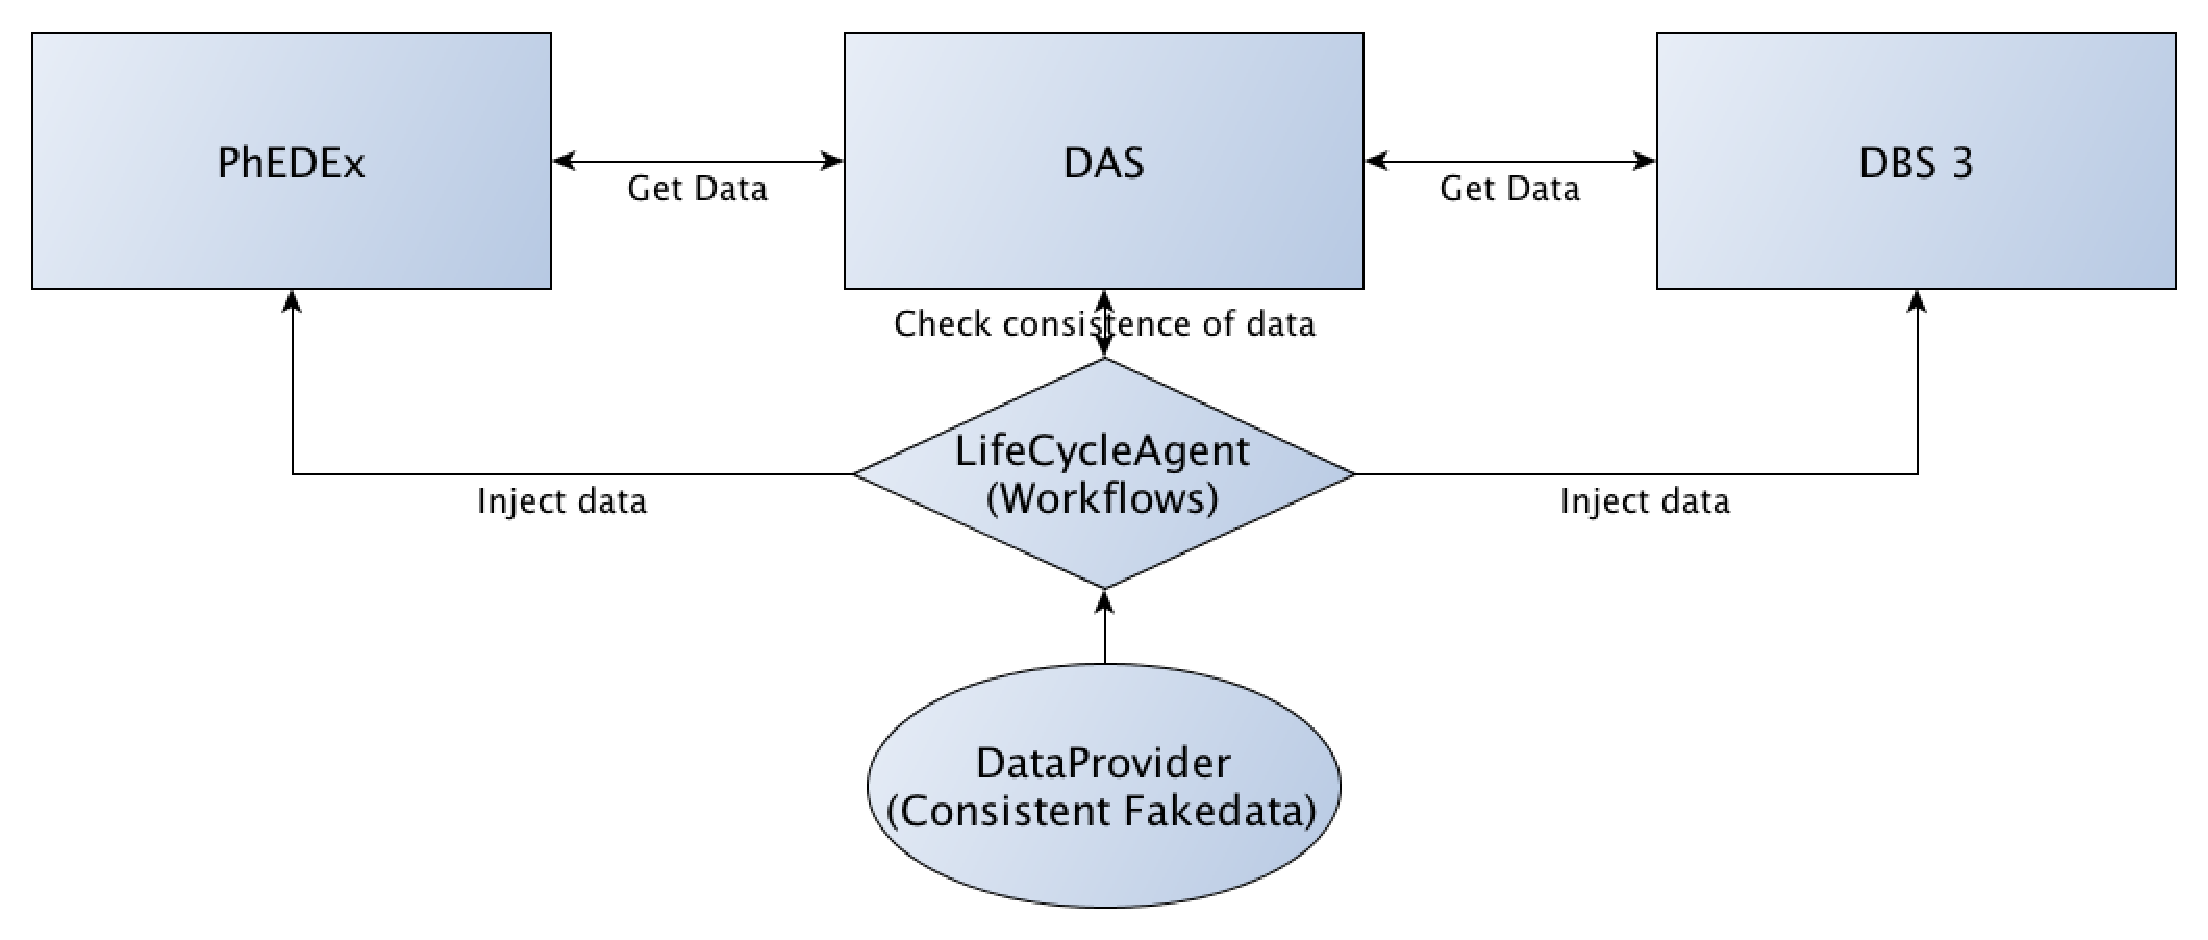
\includegraphics[width=0.8\textwidth]{IntegrationTests.pdf}
       \caption{Workflow of the integration testing of PhEDEx, DBS3, and DAS.}
 \label{fig:Integ-Phedex-DBS-DAS}
\end{figure}




